Ein \begriff{Baum} ist entweder leer oder besteht aus einer endlichen Menge von Knoten mit einem speziell ausgezeichneten Wurzelknoten (\begriff{root}) und einer endlichen Anzahl von Teilbäumen.

Ein Baum ist also rekursiv definiert und besitzt eine rekursive Datenstruktur. Wir brauchen deswegen rekursive Algorithmen zur Bearbeitung.

Der \begriff[Baum!]{Grad} ist die Anzahl der Verzweigungen nach unten. \\
Das \begriff[Baum!]{Level} ist die Anzahl der Ebenen, beginnend bei der Wurzel mit 0. \\
Die \begriff[Baum!]{Höhe} eines Baums ist die Weglänge zum weitest entfernten Knoten.

Wir wollen die Wechselbeziehung zwischen einer rekursiven Datenstruktur und einem rekursiven Algorithmus untersuchen. Dazu ist es notwendig zu wissen, dass man die Ausführung rekursiver Algorithmen als Baum darstellen kann, so zum Beispiel die \person{Fibonacci}-Zahlen. Sei dazu $F_n$ die $n$-te \person{Fibonacci}-Zahl:
\begin{center}
	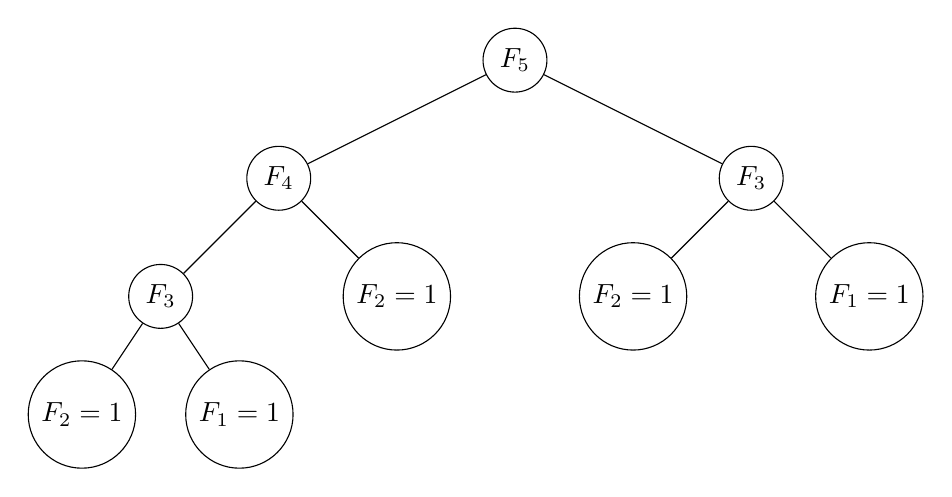
\begin{tikzpicture}[level/.style={sibling distance=60mm/#1}]
		\node[circle, draw] (root) {$F_5$}
			child {node[circle,draw] (a) {$F_4$}
				child {node[circle,draw] (b) {$F_3$}
					child {node[circle,draw] (c) {$F_2 = 1$}}
					child {node[circle,draw] (d) {$F_1 = 1$}}}
				child {node[circle,draw] (e) {$F_2 = 1$}}}
			child {node[circle,draw] (f) {$F_3$}
				child {node[circle,draw] (g) {$F_2 = 1$}}
				child {node[circle,draw] (h) {$F_1 = 1$}}};
	\end{tikzpicture}
\end{center}

Man unterscheidet dabei in die \begriff{Rechtsrekursion} und die \begriff{Linksrekursion}.
\begin{center}
	\begin{tabularx}{\textwidth}{l|l} %TODO: Tabelle bearbeiten
		\textbf{Rechtsrekursion} & \textbf{Linksrekursion} \\
		\hline
		Ein Problem $P_n$ lässt sich durch Ausführen eines Tasks $T_n$ das betrachten des Problems $P_{n-1}$ lösen. & Ein Problem $P_n$ lässt sich durch betrachten des Problems $P_{n-1}$ und anschließendes Ausführen eines Tasks $T_n$ lösen. \\
		Also lässt sich $P_n$ durch Ausführung von $T_nT_{n-1}\dots T_1T_0$ lösen. Diese Rekursion ist leicht auflösbar. Das Problem lässt sich iterativ lösen. & Also lässt sich $P_n$ durch Ausführung von $T_0T_1\dots T_{n-1}T_n$ lösen. Diese Rekursion ist nicht leicht auflösbar; sie benötigt einen Stack, da man den Speicherzustand von $T_0$ nicht aus $T_n$ vorhersagen kann.
	\end{tabularx}
\end{center}

Bei einer \begriff{allgemeinen Rekursion} sieht das Problem $P_{n,j}$  so aus.
\begin{align}
	P_{n,j} = \begin{cases}
		T_0 & n=0 \\ T_0P_{n-1,1}T_1P_{n-1,2}\dots T_{k-1}P_{n-1,k}T_k & n>0
	\end{cases} 1\le i \le k\notag
\end{align}
Auch hier genügt die Abarbeitung einem Stack!

Ein \begriff{Binärbaum} ist ein Baum mit maximalem Knotengrad 2.
\begin{itemize}
	\item maximale Anzahl an Knoten auf dem Level $l$: $2^l$
	\item maximale Anzahl Knoten auf dem gesamten Baum: $N=\sum\limits_{l=0}^h 2^l = 2^{h+1}-1$
	\item minimale Höhe eines Baums mit $N$ Knoten: $h_{min}=\lfloor\log_2 N\rfloor$
\end{itemize}

\section{Binäre Suchbäume}

Ein \begriff{binärer Suchbaum} ist ein Binärbaum, bei dem im linken Teilbaum eines Knotens nur "'kleinere'" Elemente und im rechten Teilbaum nur "'größere'" Elemente gespeichert sind. Dabei gibt es immer eine besondere Datenkomponente, die als Schlüssel (Key) dient und deren Werte eine vollständige Ordnung ermöglichen (Ordnungsrelation, typischerweise $<$).

Die elementaren Operationen auf Binärbäumen sind:
\begin{itemize}
	\item Traversieren:
	\begin{itemize}
		\item \begriff{Preorder}: $P(B)=T(B)P(B_L)P(B_R)$
		\item \begriff{Inorder}: $P(B)=P(B_L)T(B)P(B_R)$
		\item \begriff{Postorder}: $P(B)=P(B_L)P(B_R)T(B)$
		\item \begriff{Levelorder}: schichtweises Durchlaufen von oben nach unten, von links nach rechts
	\end{itemize}
	\item Einfügen und suchen: Beim Durchlaufen (Traversieren) in Inorder erhält man die in aufsteigender Schlüsselreihenfolge sortierten Elemente/Knoten(inhalte).
	\item Löschen eines Knotens mit gesuchtem Schlüsselwert im Suchbaum:
	\begin{itemize}
		\item Blatt löschen ist einfach (keine Teilbäume)
		\item Knoten hat genau einen Teilbaum: listenartige Reparatur
		\item innerer Knoten mit 2 nichtleeren Teilbäumen: 2 Möglichkeiten
		\begin{itemize}
			\item größeres Element im linken Teilbaum (des zu löschenden Knotens) suchen, dieses hat rechten Teilbaum $\Rightarrow$ diesem Knoten durch seinen linken Teilbaum ersetzen, Inhalt dieses
			(ersetzten) Elements in den „zu löschenden“ Knoten kopieren, sodann dieses größere Element (d.h. seinen Knoten) mittels 1 oder 2 löschen (Speicher freigeben!)
			\item kleines Element im rechten Teilbaum (des zu löschenden Knotens) suchen, dieses hat linken Teilbaum $\Rightarrow$ diesem Knoten durch seinen rechten Teilbaum ersetzen, Inhalt dieses (ersetzten) Elements in den „zu löschenden“ Knoten kopieren, sodann dieses kleinere Element (d.h. seinen Knoten) mittels 1 oder 2 löschen (Speicher freigeben!)
		\end{itemize}
	\end{itemize}
\end{itemize}

Ein \begriff{Sentinel} (Wachposten) ist ein Knoten, der den zu suchenden Schlüssel enthält. Alle Nullpointer eines Trees zeigen auf den Sentinel. Das sorgt dafür, dass, wenn man einen Schlüssel sucht, nach links (bei kleiner) bzw. nach rechts (bei größer) geht; ist der Wert gleich muss man nur noch schauen, ob der gefundene Wert der Sentinel ist, dann ist der gesuchte Wert nicht enthalten, andernfalls schon.